\documentclass{beamer}

%=================================================================================
% Document information
\def\firstname{Marc T.}
\def\familyname{Henry de Frahan}
\def\FileAuthor{\firstname~\familyname}
\def\FileTitle{Ways of embedding video in Beamer}
\def\FileSubject{Ways of embedding video in Beamer}
\def\FileKeyWords{\firstname~\familyname, \FileSubject, \FileTitle}

\title{\FileTitle}
\author{\FileAuthor}
\date{\today}

%=================================================================================
% Packages
\usepackage{verbatim}
\usepackage{embedfile}

%=================================================================================
% Embed the tex file into the pdf
\embedfile{\jobname}

%=================================================================================
% For media inclusion
\usepackage{multimedia}
%\usepackage{movie15}

%=================================================================================
% beamer specific
\mode<article>{\usepackage{fullpage}}
\mode<presentation>
{
  \usetheme{default}
  \usecolortheme{default} % beetle, lily, beaver
}
\setbeamertemplate{navigation symbols}{}
\setbeamertemplate{footline}{\leavevmode% 
  \hfill\hbox{% 
    \begin{beamercolorbox}[wd=.15\paperwidth,ht=2.25ex,dp=1ex,right]{date in head/foot}% 
      \scriptsize \insertframenumber{} \hspace*{2ex} 
    \end{beamercolorbox}}% 
  \vskip0pt%
}
\beamertemplatetransparentcovereddynamic
\beamertemplateballitem
\beamertemplatesolidbuttons
\usefonttheme[onlymath]{serif}
\setbeamercovered{invisible} % http://tex.stackexchange.com/questions/53860/can-i-tell-beamer-that-uncover-should-be-invisible-not-merely-grayed-out


%=================================================================================
\begin{document}
\presentation

%=================================================================================
% Title page
\frame[plain]{
  \begin{center}
    {\Huge \structure{Ways of embedding video in Beamer}}\\[2cm]
    Marc T. Henry de Frahan
  \end{center}
  \setcounter{framenumber}{0}
}

\frame{
  The full tex code is embedded in this pdf.\\
  Open the pdf in Adobe or Okular to see it.
}

 
%=================================================================================
% First way
\begin{frame}[fragile]
  \frametitle{Completely embedded, works on Linux}
  \structure{Generate a bunch of jpg pictures to make the movie}\\[0.3cm]
  \structure{Stitch them together to make the movie}\\[0.1cm]
  {\tiny
    \hspace*{1cm}\verb|mencoder mf://*.jpg -mf fps=10:type=jpg -ovc lavc -lavcopts vcodec=mpeg4:mbd=2:trell|\\
    \hspace*{1cm}\verb|        -oac copy -o output.avi|\\[0.1cm]
    \hspace*{1cm}\verb|ffmpeg -i output.avi -vcodec mpeg4 -b:v 1200k -flags +aic+mv4 output.mp4|\\[0.1cm]
    \hspace*{1cm}Do not go below 10fps for playing on Mac\\[0.3cm]
  }
  \structure{In Beamer:}\\[0.1cm]
  {\tiny
    \hspace*{1cm}\verb|\usepackage{multimedia}|\\[0.1cm]
    \hspace*{1cm}\verb|\movie{\includegraphics[width = 1.2\textheight, height = 0.9\textheight]{still.jpg}}{movie.mp4}|\\[0.3cm]
  }
  \structure{Compile PDF}\\[0.1cm]
  {\tiny
    \hspace*{1cm}\verb|pdflatex report;|\\[0.3cm]
  }
  \structure{Open PDF in Adobe X or Okular}
\end{frame}

\bgroup
\setbeamercolor{background canvas}{bg=black}
\frame[plain]{
  \frametitle{\textcolor{white}{Using multimedia package}}
  \begin{figure}
    \centering
    \hspace*{-1cm}\movie{ 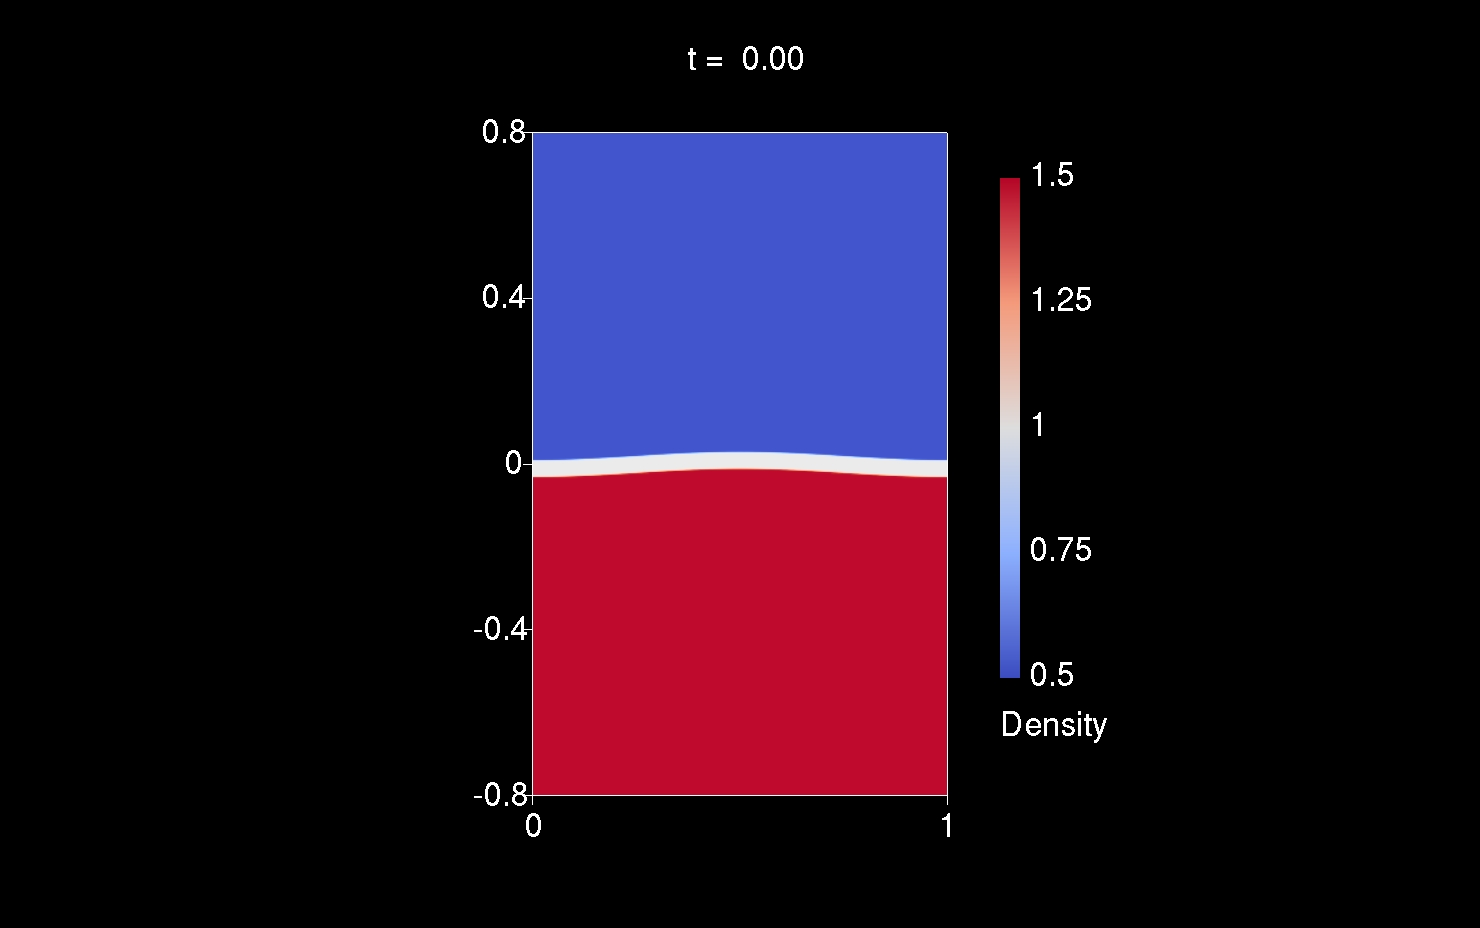
\includegraphics[width = 1.435\textheight, height = 0.9\textheight]{./movies/kh.jpg}}{./movies/kh.mp4}
  \end{figure}
}
\egroup

%=================================================================================
% Second way
\begin{frame}[fragile]
  \frametitle{Completely embedded, works on Mac,\\ not shown here, uncomment next slide}
  \structure{Generate a bunch of jpg pictures to make the movie}\\[0.3cm]
  \structure{Stitch them together to make the movie}\\[0.1cm]
  {\tiny
    \hspace*{1cm}\verb|mencoder mf://*.jpg -mf fps=10:type=jpg -ovc lavc -lavcopts vcodec=mpeg4:mbd=2:trell|\\
    \hspace*{1cm}\verb|        -oac copy -o output.avi|\\[0.1cm]
    \hspace*{1cm}\verb|ffmpeg -i output.avi -vcodec mpeg4 -b:v 1200k -flags +aic+mv4 output.mp4|\\[0.1cm]
    \hspace*{1cm}Do not go below 10fps for playing on Mac\\[0.3cm]
  }
  \structure{In Beamer:}\\[0.1cm]
  {\tiny
    \hspace*{1cm}\verb|\usepackage{movie15}|\\[0.1cm]
    \hspace*{1cm}\verb|\includemovie[poster=./still.jpg,repeat=10]{1.2\textheight}{0.9\textheight}{./movie.mp4}|\\[0.3cm]
  }
  \structure{Compile PDF}\\[0.1cm]
  {\tiny
    \hspace*{1cm}\verb|pdflatex report;|\\[0.3cm]
  }
  \structure{Open PDF in Adobe X}
\end{frame}

%% \bgroup
%% \setbeamercolor{background canvas}{bg=black}
%% \frame[plain]{
%%   \frametitle{\textcolor{white}{Using movie15 package}}
%%   \begin{figure}
%%     \centering
%%     \hspace*{-1cm}\includemovie[poster=./movies/kh.jpg,repeat=10]{1.435\textheight}{0.9\textheight}{./movies/kh.mp4}
%%   \end{figure}
%% }
%% \egroup


%=================================================================================
% Third way
\begin{frame}[fragile]
  \frametitle{Open in external viewer, works on Linux/Windows}
  \structure{Generate a bunch of jpg pictures to make the movie}\\[0.3cm]
  \structure{Stitch them together to make the movie}\\[0.1cm]
  {\tiny
    \hspace*{1cm}\verb|mencoder mf://*.jpg -mf fps=10:type=jpg -ovc lavc -lavcopts vcodec=mpeg4:mbd=2:trell|\\
    \hspace*{1cm}\verb|        -oac copy -o output.avi|\\[0.1cm]
    \hspace*{1cm}\verb|mencoder 'mf://*.jpg' -mf type=jpg:fps=10 -ovc lavc -lavcopts vcodec=wmv2|\\
    \hspace*{1cm}\verb|        -oac copy -o output.mpg|\\[0.1cm]
    \hspace*{1cm}Do not go below 10fps for playing on Mac\\[0.3cm]
  }
  \structure{In Beamer:}\\[0.1cm]
  {\tiny
    \hspace*{1cm}\verb|\usepackage{multimedia}|\\[0.1cm]
    \hspace*{1cm}\verb|\movie[externalviewer]{\includegraphics[width = 1.2\textheight, height = 0.9\textheight]{still.jpg}}{movie.mpg}|\\[0.3cm]
  }
  \structure{Compile PDF}\\[0.1cm]
  {\tiny
    \hspace*{1cm}\verb|pdflatex report;|\\[0.3cm]
  }
  \structure{Open PDF, make sure you fix fullscreen permissions}
\end{frame}


\begin{frame}
  \frametitle{Using external viewer (with multimedia package)}
  \begin{center}
    \movie[externalviewer]{ 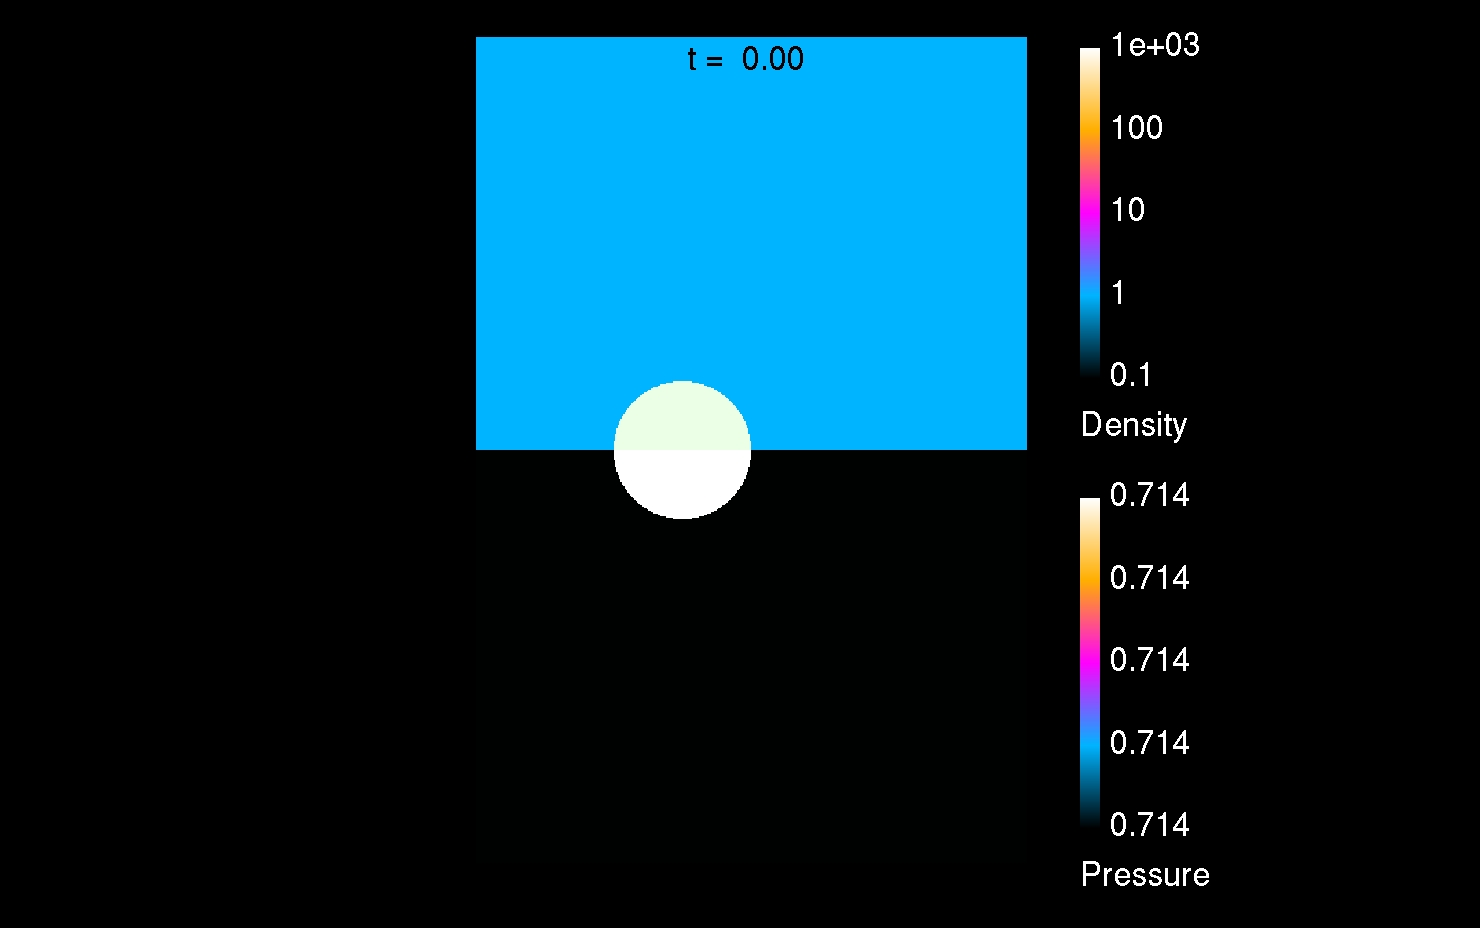
\includegraphics[width = 0.8\textwidth]{./movies/sd000.jpg}}{./movies/sd.mpg} 
  \end{center}
\end{frame}



\end{document}
